\documentclass[tikz,border=12pt]{standalone}
\usepackage[T1]{fontenc}
\usepackage{mathpazo}
\usepackage{amsmath,amssymb}
\usepackage{pgfplots}
\usepgfplotslibrary{groupplots}
\pgfplotsset{compat=1.18}

\definecolor{stblue}{HTML}{7B97AD}
\definecolor{rwgold}{HTML}{B8995E}
\definecolor{sage}{HTML}{7A9A7E}
\definecolor{dkbrown}{HTML}{3D3530}
\definecolor{wmgray}{HTML}{7B7067}
\definecolor{cream}{HTML}{F9F6F0}
\definecolor{border}{HTML}{D4C9B8}
\definecolor{terracotta}{HTML}{C47A6A}
\definecolor{lavender}{HTML}{907EA0}

\begin{document}
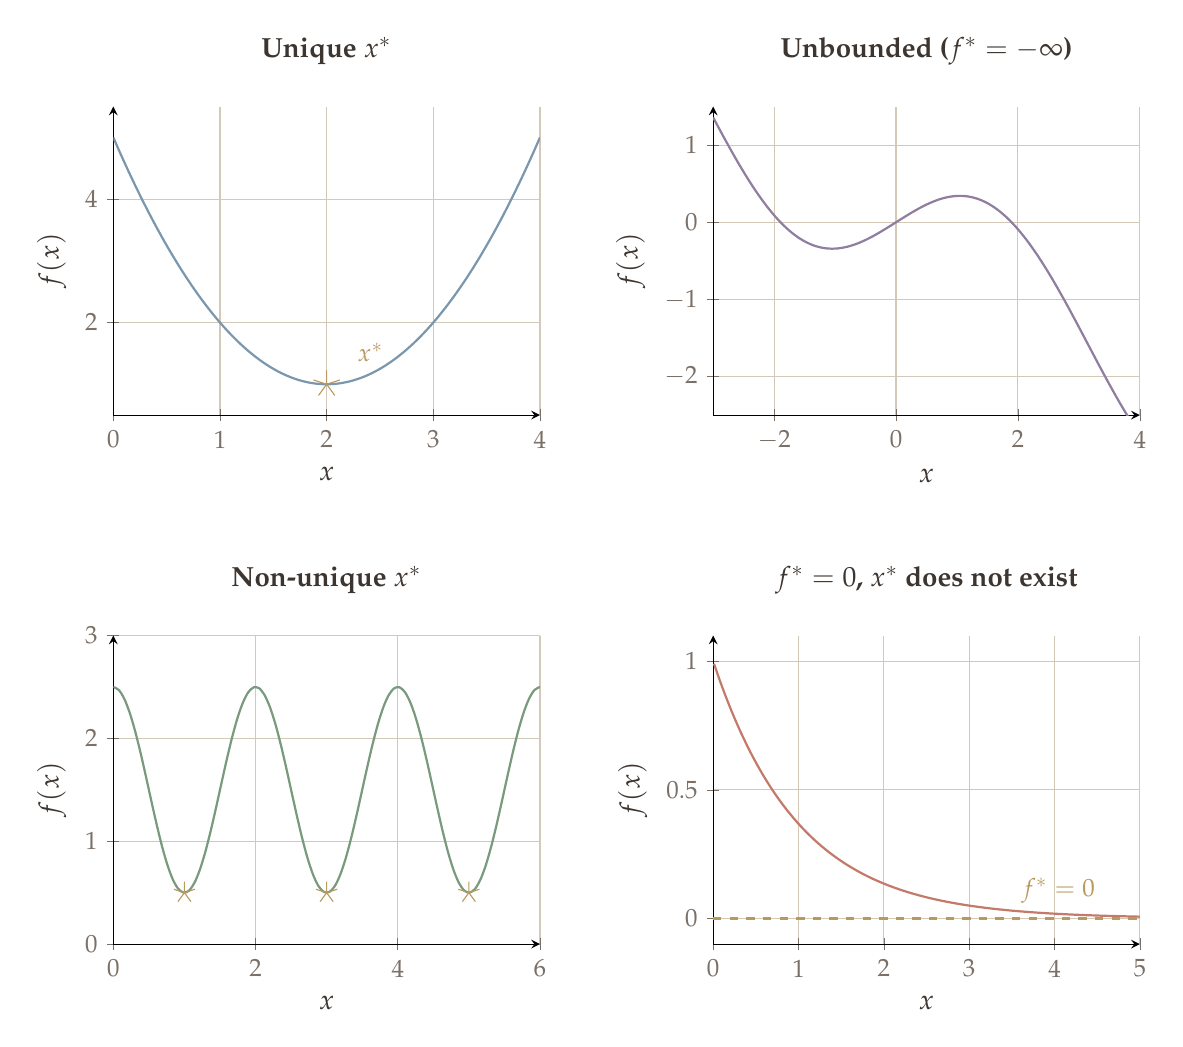
\begin{tikzpicture}
\begin{groupplot}[
  group style={
    group size=2 by 2,
    horizontal sep=2.2cm,
    vertical sep=2.8cm,
  },
  width=7cm, height=5.5cm,
  axis lines=left,
  every axis label/.style={font=\normalsize, color=dkbrown},
  every tick label/.style={font=\small, color=wmgray},
  grid=major,
  grid style={border, thin},
  tick style={wmgray},
  title style={font=\normalsize\bfseries, color=dkbrown, at={(0.5,1.05)}},
]

% Panel 1: Unique x*
\nextgroupplot[title={Unique $x^*$}, xmin=0, xmax=4, ymin=0.5, ymax=5.5,
  xlabel={$x$}, ylabel={$f(x)$}]
\addplot[stblue, thick, smooth, domain=0:4, samples=80] {(x-2)^2 + 1};
\addplot[only marks, mark=star, mark size=5pt, rwgold, mark options={fill=rwgold}]
  coordinates {(2,1)};
\node[rwgold, font=\small, anchor=south west] at (axis cs:2.2,1.2) {$x^*$};

% Panel 2: Unbounded (f*=-inf)
\nextgroupplot[title={Unbounded ($f^* = -\infty$)}, xmin=-3, xmax=4, ymin=-2.5, ymax=1.5,
  xlabel={$x$}, ylabel={$f(x)$}]
\addplot[lavender, thick, smooth, domain=-3:4, samples=80] {-0.5*x + sin(deg(x))};

% Panel 3: Non-unique x*
\nextgroupplot[title={Non-unique $x^*$}, xmin=0, xmax=6, ymin=0, ymax=3,
  xlabel={$x$}, ylabel={$f(x)$}]
\addplot[sage, thick, smooth, domain=0:6, samples=80] {cos(deg(pi*x)) + 1.5};
\addplot[only marks, mark=star, mark size=4pt, rwgold, mark options={fill=rwgold}]
  coordinates {(1,0.5) (3,0.5) (5,0.5)};

% Panel 4: Infimum not attained
\nextgroupplot[title={$f^* = 0$, $x^*$ does not exist}, xmin=0, xmax=5, ymin=-0.1, ymax=1.1,
  xlabel={$x$}, ylabel={$f(x)$}]
\addplot[terracotta, thick, smooth, domain=0.01:5, samples=80] {exp(-x)};
\draw[rwgold, dashed, line width=0.8pt] (axis cs:0,0) -- (axis cs:5,0);
\node[rwgold, font=\small, anchor=south west] at (axis cs:3.5,0.02) {$f^* = 0$};

\end{groupplot}
\end{tikzpicture}
\end{document}
